%-----------------------------------------------
% Template para criação de resumos de projectos/dissertação
% jlopes AT fe.up.pt,   Fri Jul  3 11:08:59 2009
%-----------------------------------------------

\documentclass[9pt,a4paper]{extarticle}

%% English version: comment first, uncomment second
%\usepackage[portuguese]{babel}  % Portuguese
\usepackage[english]{babel}     % English
\usepackage{graphicx}           % images .png or .pdf w/ pdflatex OR .eps w/ latex
\usepackage{times}              % use Times type-1 fonts
\usepackage[utf8]{inputenc}     % 8 bits using UTF-8
\usepackage{url}                % URLs
\usepackage{multicol}           % twocolumn, etc
\usepackage{float}              % improve figures & tables floating
\usepackage[tableposition=top]{caption} % captions
%% English version: comment first (maybe)
\usepackage{indentfirst}        % portuguese standard for paragraphs
%\usepackage{parskip}

%% page layout
\usepackage[a4paper,margin=30mm,noheadfoot]{geometry}

%\graphicspath{{figures/}}

%% space between columns
\columnsep 12mm

%% headers & footers
\pagestyle{empty}

%% figure & table caption
\captionsetup{figurename=Fig.,tablename=Tab.,labelsep=endash,font=bf,skip=.5\baselineskip}

%% heading
\makeatletter
\renewcommand*{\@seccntformat}[1]{%
  \csname the#1\endcsname.\quad
}
\makeatother

%% avoid widows and orphans
\clubpenalty=300
\widowpenalty=300

\begin{document}

\title{\vspace*{-8mm}\textbf{\textsc{Reverse Engineering of Interaction Patterns}}}
\author{\emph{Clara Raquel da Costa e Silva Sacramento}\\[2mm]
\small{Dissertação developed under the supervision of \emph{Prof.\ Ana Paiava}}\\
\small{at \emph{Faculdade de Engenharia da Universidade do Porto}}}
\date{}
\maketitle
%no page number 
\thispagestyle{empty}

\vspace*{-4mm}\noindent\rule{\textwidth}{0.4pt}\vspace*{4mm}

\begin{multicols}{2}

\section{Context}\label{sec:context}

%Neste documento apresentam-se alguns conselhos e instruções para a preparação dos resumos de projecto/dissertação. Pede-se aos autores o favor de, dentro do possível, cumprirem com as instruções que são dadas, assim como com a estrutura apresentada, de forma a manter-se o mesmo aspecto em todos os resumos. Nas sub-secções~\ref{sec:lingua} a ~\ref{sec:number} podem encontrar-se alguns detalhes sobre a formatação do documento. Na secção ``Motivação'' deve ser apresentado o enquadramento do trabalho, dando ideia das necessidades que o mesmo cobre.

Web applications are getting more and more important. Due to their stability and security against losing data, there is a growing trend to move applications towards the Web, with the most notorious examples being Google's mail and office software applications. Web applications can now handle tasks that before could only be performed by desktop applications, like editing images or creating spreadsheet documents.

Despite the relevance that Web applications have in the community, they still suffer from a lack of standards and conventions, unlike desktop and mobile applications. This means that the same task can be implemented in many different ways, which makes automated testing difficult to accomplish and inhibits reuse of testing code. For instance, authentication (\textit{login}) failure usually triggers the appearance of an error message, but some implementations simply erase the inserted data, with no error message visible.

GUIs \textit{(Graphical User Interfaces)} of all kinds are populated with recurring behaviors that vary slightly; examples being the already mentioned authentication via \textit{login/password} pair and content search. These behaviors (patterns) are called User Interface (UI) patterns, and are recurring solutions to common design problems. Due to their widespread use, UI patterns allow users a sense of familiarity and comfort when using Web applications.

However, while UI patterns are familiar to users, their implementation may vary significantly; but it is possible to define generic and reusable test strategies (User Interface Test Patterns - UITP) to test those patterns. This requires a configuration process, in order to adapt the tests to different applications.

A great deal of effort in model-based testing is related to the creation of the model. In addition, the model itself, while a powerful tool of abstraction, can have conceptual errors, unknowingly introduced by the tester. These problems can be reduced by generating those models automatically via reverse engineering. 

\section{Motivation}\label{sec:motiva}

This dissertation aims to continue the work done on PARADIGM-RE, a component of the PBGT \textit{(Pattern-based GUI Testing)} project responsible for extracting part of the Web application model from the Web application itself via reverse engineering, by developing a completely new tool to extract a partial model of a Web application via reverse engineering. 

\section{Goals}\label{sec:goals}

%A secção ``Objectivos'' deve enunciar claramente os objectivos a atingir com o trabalho de projecto/dissertação, enquadrando-os na respectiva área de actividade a que o trabalho se destina. 
%Por exemplo, este documento tem como objectivos:
%\begin{itemize}
%\item Servir de modelo/exemplo do ponto de vista da dos resumos;
%\item Apresentar o aspecto gráfico que se pretende para os resumos;
%\item Disponibilizar \emph{templates} a quem pretenda utilizar \LaTeX.
%\end{itemize}

The major goals for this dissertation are: to improve the existing reverse engineering and pattern inferring process and its inferring accuracy, remove the need for user interaction, and automate the model construction; or in other words, independently/automatically explore a Web application, infer the existing UI patterns in its pages, and finally produce a model with the UI Test Patterns that define the strategies to test the UI Patterns present in the web application. This is meant to speed up model construction, spare work to the tester, and mitigate the number of errors introduced into the model.

\section{Description of the Approach}\label{sec:work}
This dissertation presents a dynamic reverse engineering approach that aims to extract part of the model of an existing Web application through the identification of User Interface (UI) patterns. This approach explores automatically any Web application, records information related to the interaction, analyzes the gathered information, tokenizes it, and infers the existing UI patterns via syntactical analyzing. After complemented with additional information and validated, the model extracted is the input for the PBGT approach to test the web application under analysis.

\subsection{PBGT Overview}\label{sec:pbgt}

As mentioned before, the focus of this dissertation is PARADIGM-RE, the reverse engineering component of a research project named PBGT. The goal of this project is to develop a model-based GUI testing approach embodied in a test supporting tool, that can be used in industrial contexts.

The PBGT tool has main five components: \textbf{PARADIGM}, a DSL (\textit{Domain Specific Language}) to define GUI testing models based on UI Test Patterns; \textbf{PARADIGM-RE}, a Web application reverse engineering tool whose purpose is to extract UI patterns from Web pages without access to their source code, and use that information to generate a test model written in PARADIGM; \textbf{PARADIGM-ME}, a modeling and testing environment, built to support the creation of test models; \textbf{PARADIGM-TG}, an automatic test case generation tool that generates test cases from test models defined in PARADIGM according to coverage criteria selected by the tester; and finally, a test case execution tool, named \textbf{PARADIGM-TE}, which executes test cases, analyzes their coverage with a coverage analysis tool named \textbf{PARADIGM-COV}, and returns detailed execution reports.

\subsection{UI Patterns and UI Test Patterns}

A UI Test Pattern defines a test strategy to test a specific UI pattern, which is formally defined by a set of test goals (for later configuration) with the form $< Goal; V; A; C; P >$. 

\textit{Goal} is the \textit{ID} of the test. \textit{V} is a set of pairs { [\textit{variable}, \textit{inputData}] } relating test input data with the variables involved in the test. \textit{A} is the sequence of actions to perform during test case execution. \textit{C} is the set of possible checks to perform during test case execution, for example, “check if it remains in the same page”. \textit{P} is a Boolean expression (precondition) defining the set of states in which it is possible to execute the test. 

The UI Patterns defined in the PARADIGM language are: \textbf{Login} (this pattern consists of two input fields (a normal input box for email or username, and a cyphered text for the password) and a submit button, with optionally a ``remember me'' checkbox); \textbf{Find} (this pattern consists of one or more input fields, where the user inserts keywords to search, and a submit button to start the search); \textbf{Sort} (this pattern sorts a list of data by a common attribute (e.g., price, name, relevance, etc.) according to a defined criteria (ascending or descending, alphabetically, etc.)); \textbf{Master Detail} (this pattern is present in a web page when selecting an element from a set (called \textit{master}) results in filtering/updating another related set (called \textit{detail}) accordingly); \textbf{Input} (this pattern is any kind of element in which text can be inserted); and \textbf{Call} (this pattern is any kind of element where a click triggers some procedure that may result in a change of page).
\subsection{Previous Tool}
The  approach developed in this dissertation aims to improve on the process developed on the previous work \cite{nabuco2013inferring} done on the PARADIGM-RE tool. In particular it aims to be fully automatic. The previous tool required the intervention of the user to interact with the Web application under analysis in order to save the interaction traces and proceed from there. It extracted information from an user's interaction with the Web application under analysis, analyzed the information, produced some metrics (such as the total ratio of the LOC (\textit{lines of code}), length of all visited pages and the ratio of two subsequent pages), and finally used those metrics and the user interaction's information to infer UI patterns via a set of heuristic rules. 

\subsection{Architecture}

The architecture of the tool is seen in Figure \ref{fig:retool}. The approach can be divided into three parts: \textbf{WebsiteExplorer}, \textbf{LogProcessor}, and \textbf{PatternInferrer}.
\begin{figure}[H]
\centerline{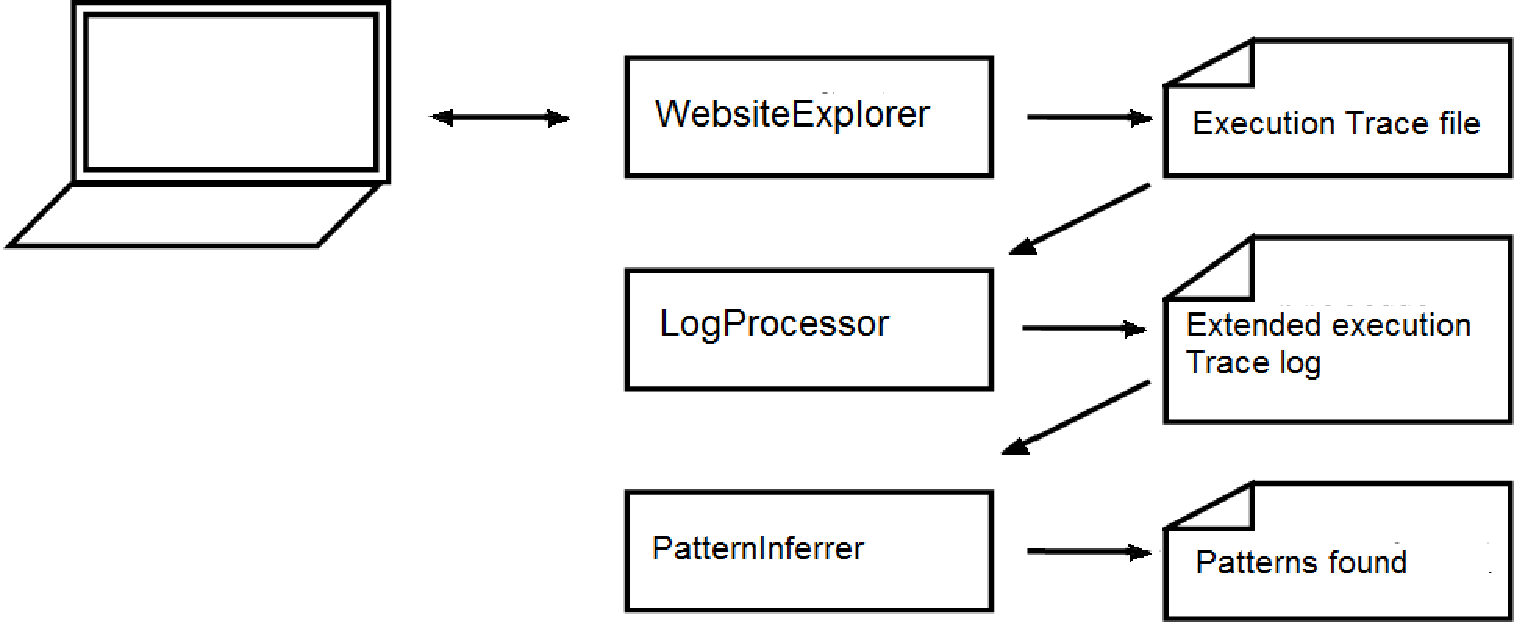
\includegraphics[scale=.3]{retool}}
\caption{The architecture of the approach.}
\label{fig:retool}
\end{figure}
\textbf{WebsiteExplorer} loads user configurations (which can modify almost all components of the tool), interacts automatically with the AUT and produces an execution trace file with the actions taken. \textbf{LogProcessor} is a text parser. It analyzes the previous file, parses each line, searches for important keywords, uses them to identify the action contained in the line, and produces an updated execution trace file. Finally, \textbf{PatternInferrer} analyzes the updated execution file, identifies the existent patterns, their location in the website and any existing parameters, and produces an XML file with the results, the exceptions being the \textbf{Menu} and \textbf{MasterDetail} patterns. Since the explorer cannot be relied on to explore every element belonging to these patterns in each page, elements belonging to these patterns are found through analyzing the current page source and extracting all elements that obey a set of rules (which can be changed in the user configurations and loaded to the tool).

The patterns identifiable by this tool are all of those defined in the PARADIGM language, plus the \textbf{Menu} UI pattern (a collection of navigational links inside a page, usually organized in a tree structure), which is going to be included in the PARADIGM DSL in the future. 

\section{Conclusions}\label{sec:conclusion}
This dissertation aims to continue the work done on PARADIGM-RE, a tool responsible for extracting part of the Web application model from the Web application itself via reverse engineering.
The previous tool requires user interaction to explore a Web application, analyzes the execution trace file, HTML source and URLs  of all pages visited, and infers patterns through a set of heuristic rules; the current tool is fully automatic, requires only the execution trace file, and infers patterns through syntactical analysis of a previously tokenized execution trace file, and for some patterns, the analysis of the source code.

%%English version: comment first, uncomment second
%\bibliographystyle{unsrt-pt}  % numeric, unsorted refs
\bibliographystyle{unsrt}  % numeric, unsorted refs
\bibliography{myrefs}

\end{multicols}

\end{document}
